% Le titre de la partie
\section{La pratique des réseaux de neurones artificiels}

%%%%%%%%%%%%%%%%%%%%%%%%%%%%%%%%%%%%%%%%%%%%%%%%
% Première diapo
%%%%%%%%%%%%%%%%%%%%%%%%%%%%%%%%%%%%%%%%%%%%%%%%

\begin{frame}
\frametitle{Création de la base de données}
\framesubtitle{Données réelles}

\begin{columns}
\begin{column}{6.8cm}
    \begin{itemize}
        \item<1->   Chercher des images sur Internet.
        \begin{itemize}
            \item<1->   Google et quelques sites web.
        \end{itemize}
        %Quantité trés faible d'images sur internet
        \item<1->   Prendre des photos de la rue.
        \begin{itemize}
            \item<1->   Parkings publics.
        \end{itemize}
        %Problèmes d'autorisation et de nécéssité d'explication
        \item<2->   Écire un programme d'annotation.
        %Permettant l'annotation en des fichiers texte contenant les coordonnées des plaques
        \item<2->   Annoter les images collectées.
    \end{itemize}
\end{column}
\begin{column}{6cm}
    \begin{figure}
        \begin{overprint}
            \captionsetup{justification=centering}
            \onslide<1>\centering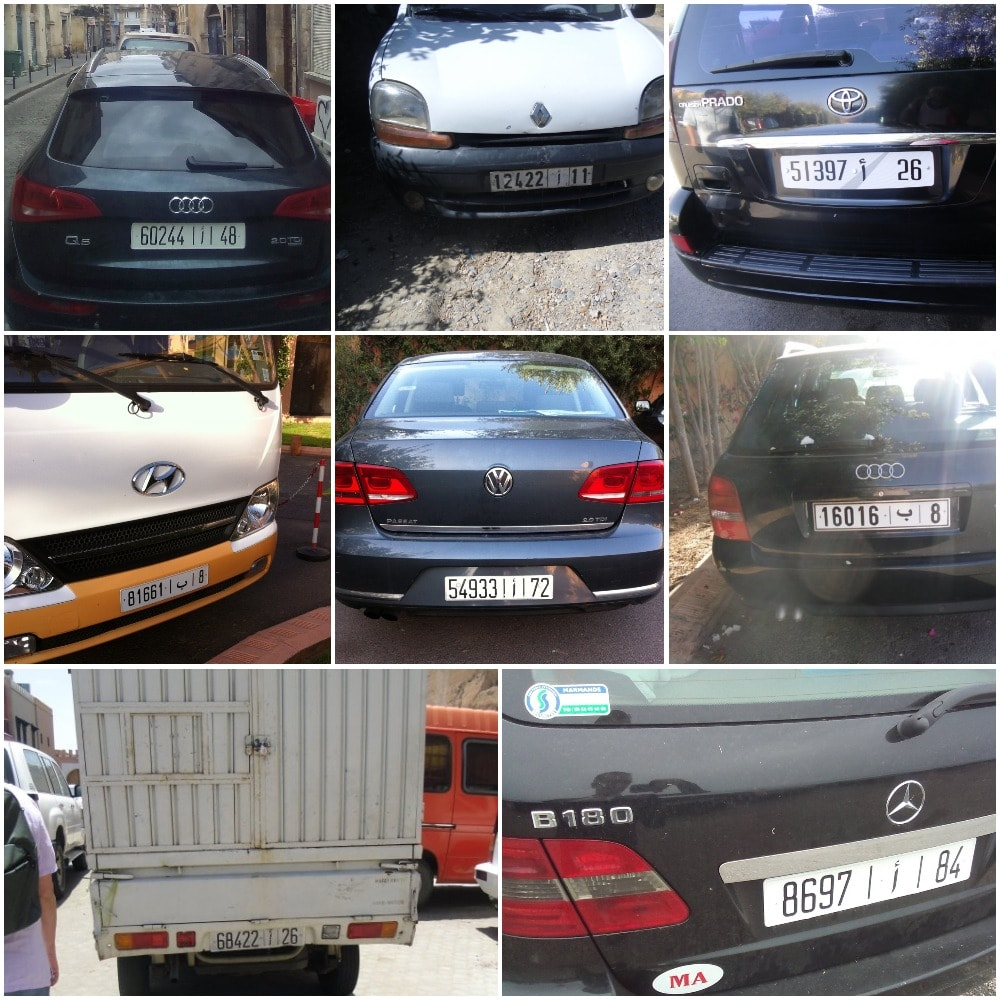
\includegraphics[width=0.8\textwidth]{figures/Data_real.PNG}\caption{Exemples d'images collectées}
            \onslide<2>\centering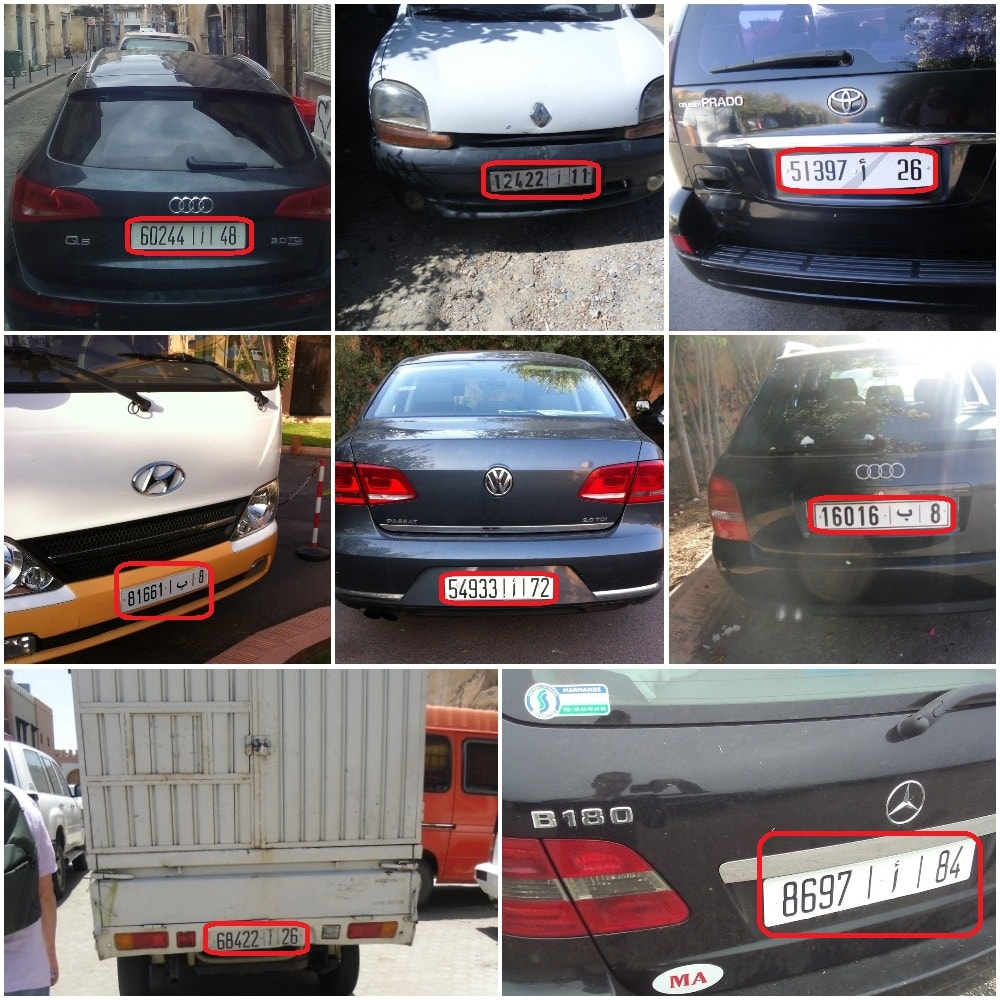
\includegraphics[width=0.8\textwidth]{figures/Data_ann.PNG}\caption{Exemples d'images annotées}
        \end{overprint}
    \end{figure}
\end{column}
\end{columns}

\end{frame}


%%%%%%%%%%%%%%%%%%%%%%%%%%%%%%%%%%%%%%%%%%%%%%%%
% Deuxième diapo
%%%%%%%%%%%%%%%%%%%%%%%%%%%%%%%%%%%%%%%%%%%%%%%%

\begin{frame}
\frametitle{Création de la base de données}
\framesubtitle{Données synthétisées}

\begin{columns}
\begin{column}{6cm}
    \begin{itemize}
        \item<1->   Analyser les caractéristiques des plaques marocaines.
        \item<2->   Trouver une base de données d'images sans plaques.
        \item<3->   Écrire un programme qui génère des données annotées.
        \item<4->   Analyser et optimiser la qualité des données générées.
    \end{itemize}
\end{column}
\begin{column}{6cm}
    \begin{figure}
        \begin{overprint}
            \onslide<1>\centering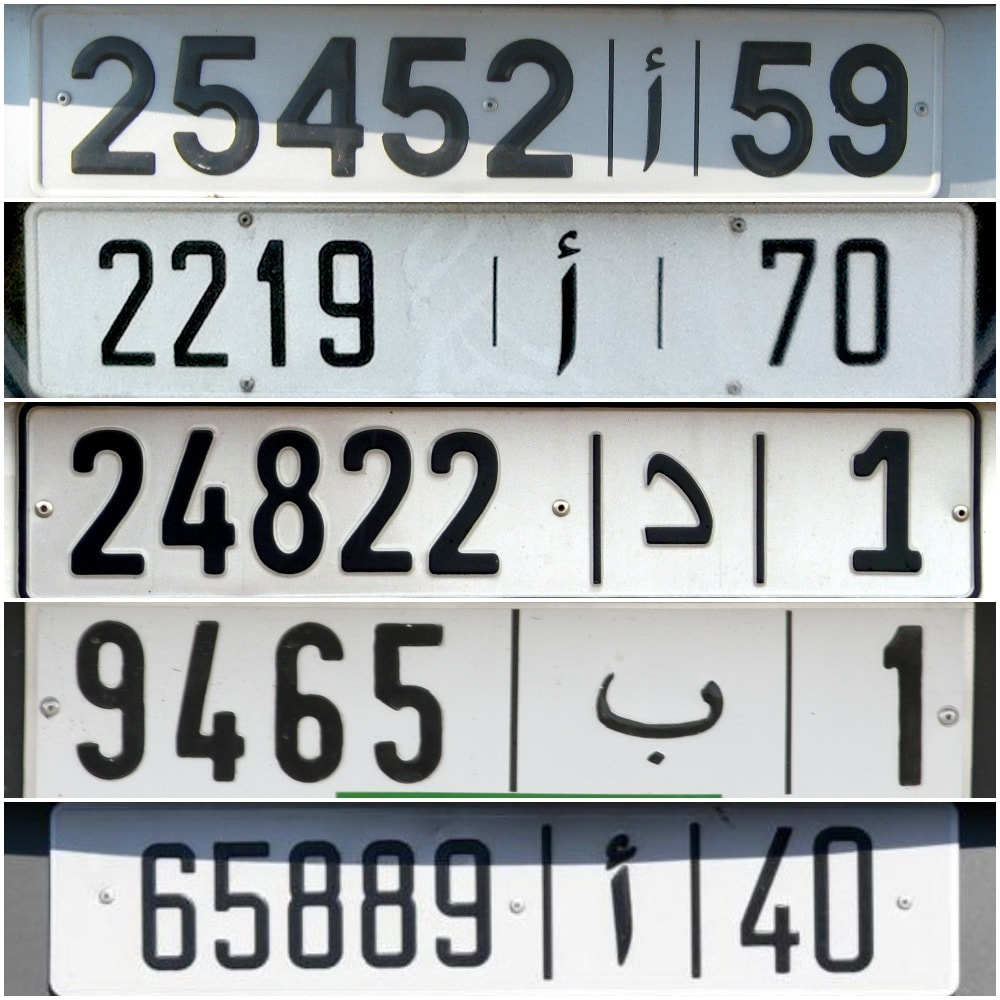
\includegraphics[width=0.8\textwidth]{figures/Plaques.PNG}\caption{Exemples de plaques maroccaines}
            \onslide<2>\centering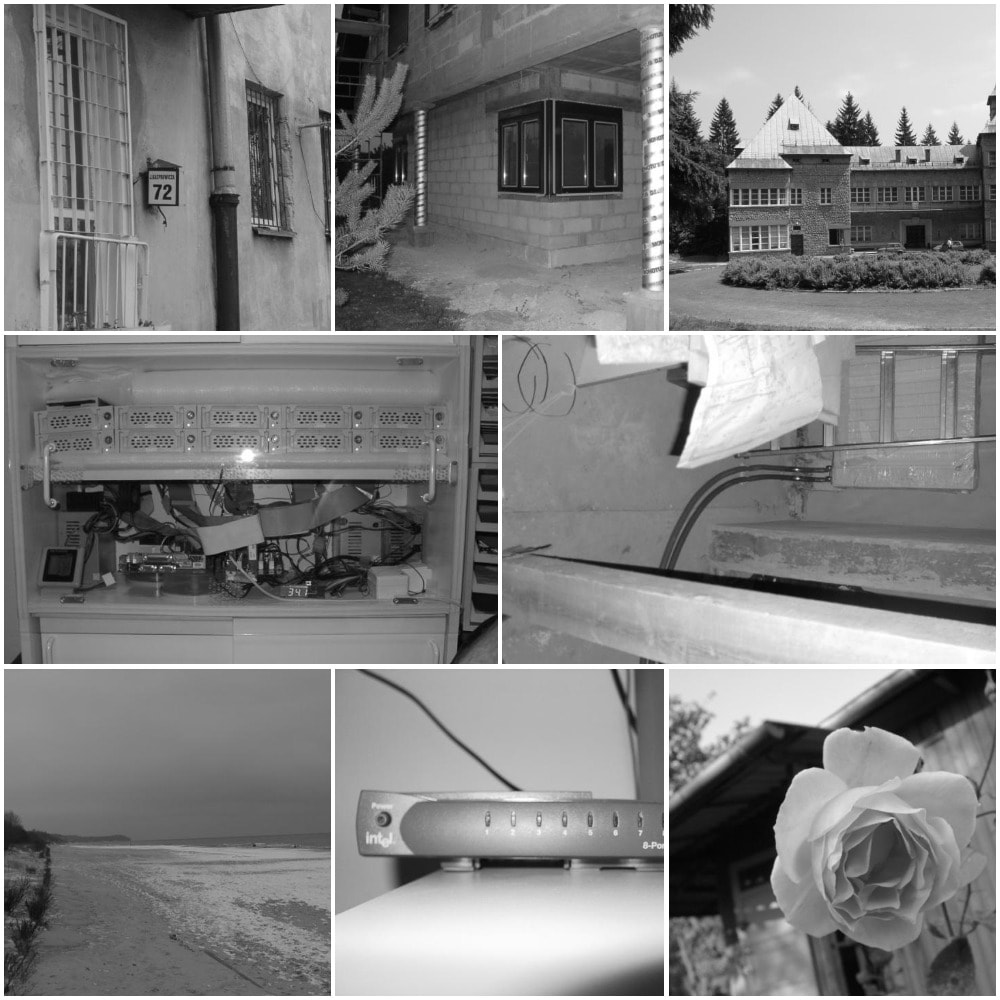
\includegraphics[width=0.8\textwidth]{figures/SUN_data.PNG}\caption{Exemples d'images sans plaques}
            \onslide<3>\centering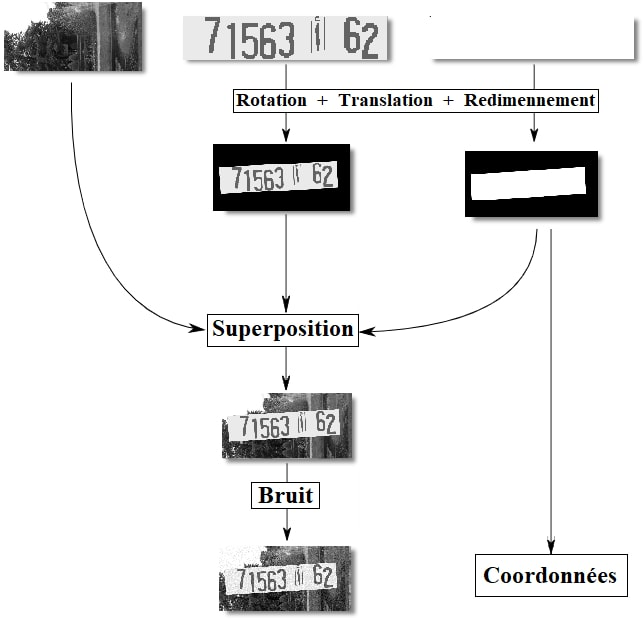
\includegraphics[width=0.8\textwidth]{figures/Gen_process.PNG}\caption{Le processus des génération de données annotées}
            \onslide<4>\centering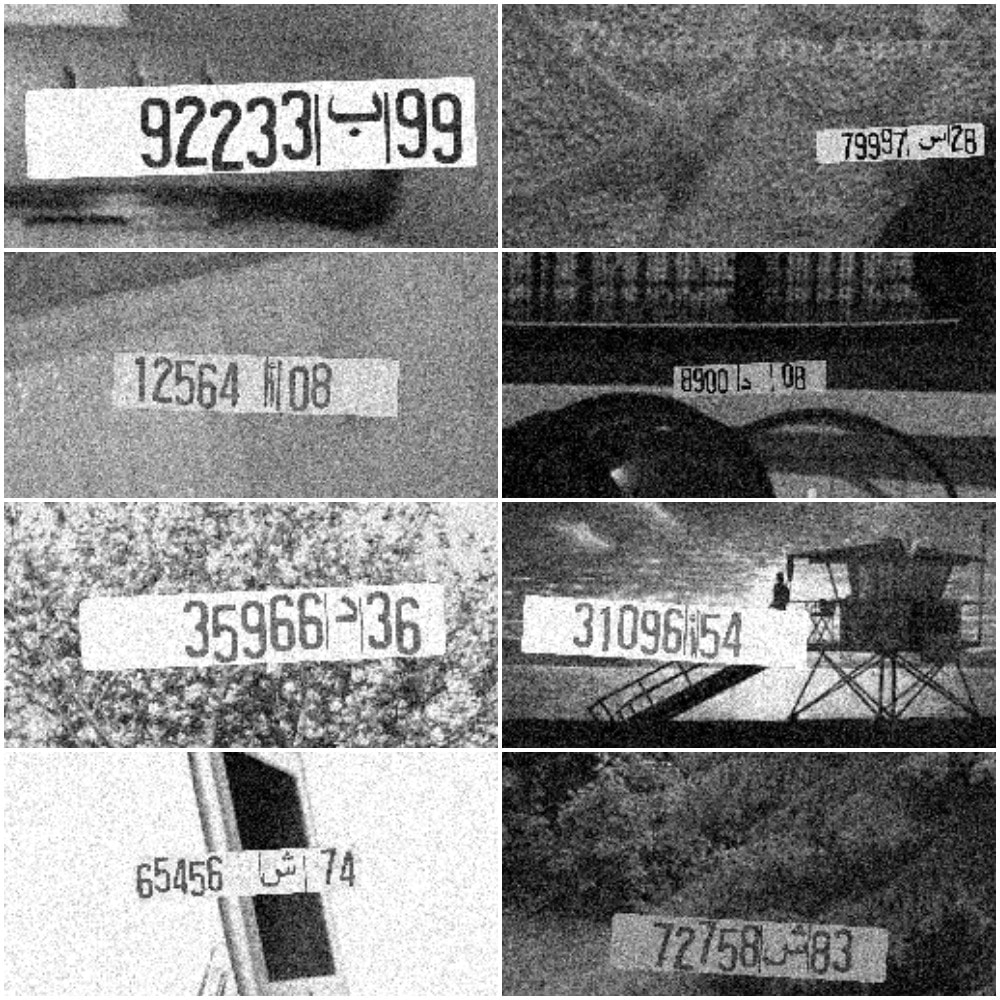
\includegraphics[width=0.8\textwidth]{figures/Data_gen.PNG}\caption{Exemples des données générées}
        \end{overprint}
    \end{figure}
\end{column}
\end{columns}
\end{frame}


%%%%%%%%%%%%%%%%%%%%%%%%%%%%%%%%%%%%%%%%%%%%%%%%
% Troisième diapo
%%%%%%%%%%%%%%%%%%%%%%%%%%%%%%%%%%%%%%%%%%%%%%%%

\begin{frame}
\frametitle{Création de la base de données}
\framesubtitle{Comparaison entre bases de données}
\begin{table}

\begin{tabular}{c|c|c|c}
    Type de données  &  Moyenne  &  Ecart type &  Coefficient de variation \\
    \hline
    Générées         &  126      &  32.71      &  3.86  \\
    Réelles          &  97.84    &  24.79      &  3.94
\end{tabular}
\end{table}
\centering
\begin{figure}
    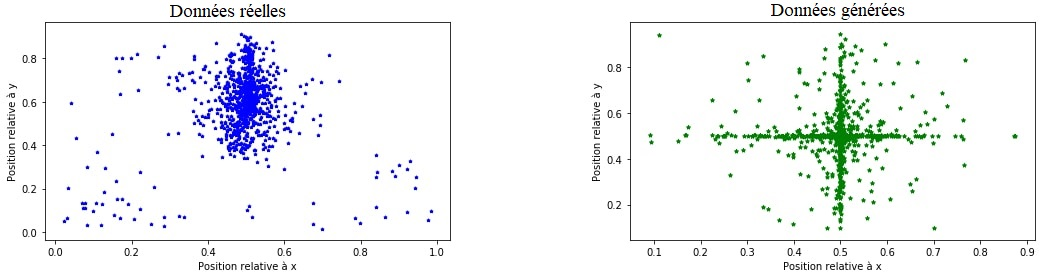
\includegraphics[width=1\textwidth]{figures/Data_dispers.PNG}\caption{Dispersion des centres des plaques}
\end{figure}
\end{frame}

%%%%%%%%%%%%%%%%%%%%%%%%%%%%%%%%%%%%%%%%%%%%%%%%
% Quatrième diapo
%%%%%%%%%%%%%%%%%%%%%%%%%%%%%%%%%%%%%%%%%%%%%%%%

\begin{frame}
\frametitle{Création du réseau de neurones}
\framesubtitle{Un problème de régression ?}
\begin{columns}
\begin{column}{6.5cm}
    \begin{itemize}
        \item<1->   Un model simple de prédiction.
        \item<2->   Prédictions érronées.
        \item<2->   Problème de "Surapprentissage" .
    \end{itemize}
\end{column}
\begin{column}{6cm}
    \begin{figure}
        \begin{overprint}
            \onslide<1>\centering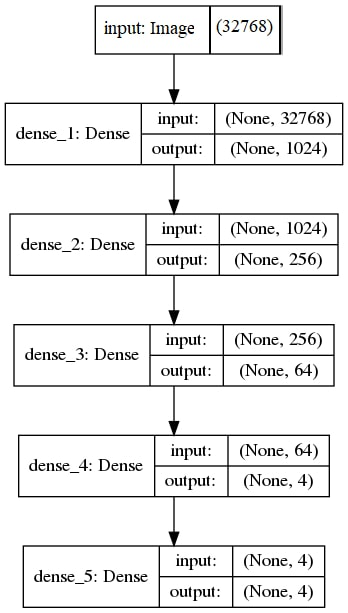
\includegraphics[width=0.5\textwidth]{figures/Model_1.PNG}\caption{Model de régression}
            \onslide<2>\centering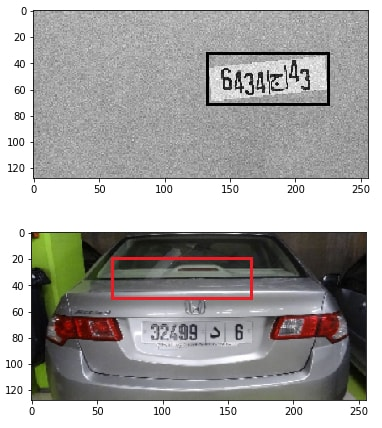
\includegraphics[width=0.7\textwidth]{figures/Resultats_1.PNG}\caption{Resultats des prédictions du réseau}
        \end{overprint}
    \end{figure}
\end{column}
\end{columns}
\end{frame}

%%%%%%%%%%%%%%%%%%%%%%%%%%%%%%%%%%%%%%%%%%%%%%%%
% Cinquième diapo
%%%%%%%%%%%%%%%%%%%%%%%%%%%%%%%%%%%%%%%%%%%%%%%%

\begin{frame}
\frametitle{Création du réseau de neurones}
\framesubtitle{Un problème de classification ?}

\begin{itemize}
    \item<1->   Problème : Dimentionnalité élevée du problème .
    %Une des solutions consiste à remplacer les données originales par des données dans un espace de plus de petite dimension, tout en conservant l'essentiel des caractéristiques de celles-ci. C'est la réduction de la dimensionnalité. Deux approches classiques sont la sélection de caractéristique, qui consiste à choisir un petit ensemble de variables représentatives, et l'extraction de caractéristique, qui consiste à définir de nouvelles variables plus pertinentes.
    \item<2->   Idée : Extraction de caractéristiques.
    \item<3->   Solution : Réseaux de neurones convolutionnels.
    \item<4->   Inconvenient : Traitement de chaque région dans l'image.
\end{itemize}

\centering
\begin{figure}
    \begin{overprint}
        \captionsetup{justification=centering}
        \onslide<1>\centering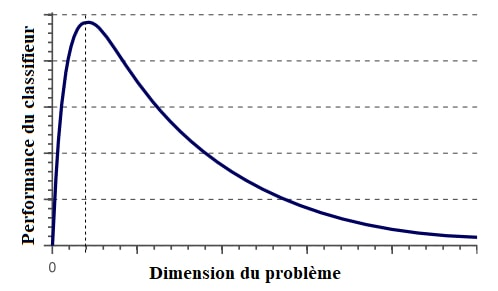
\includegraphics[width=0.55\textwidth]{figures/Malediction.PNG}\caption{Malédiction de la dimensionnalité}
        \onslide<2>\centering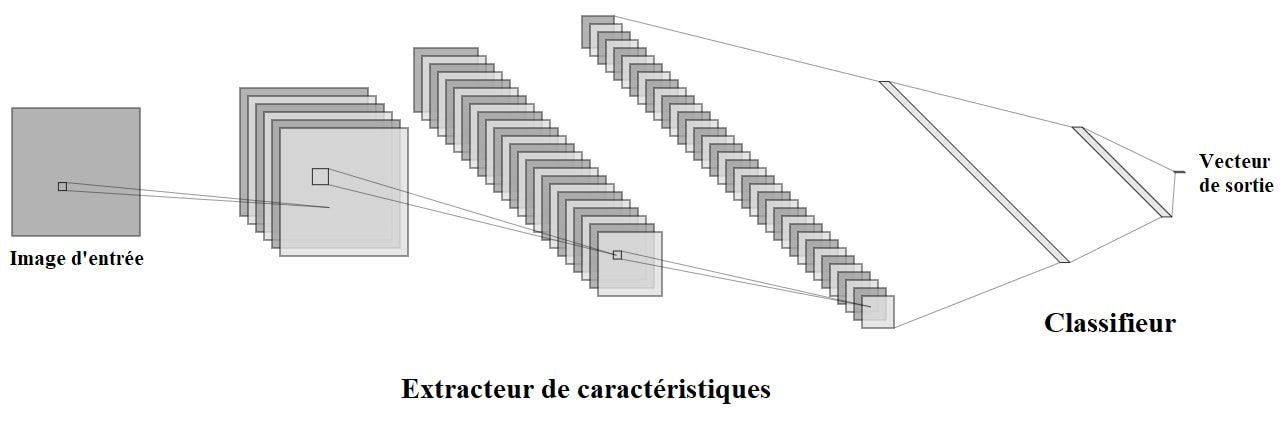
\includegraphics[width=0.95\textwidth]{figures/Extracteur.PNG}\caption{Principe de l'extraction des caracteristiques}
        \onslide<3>\centering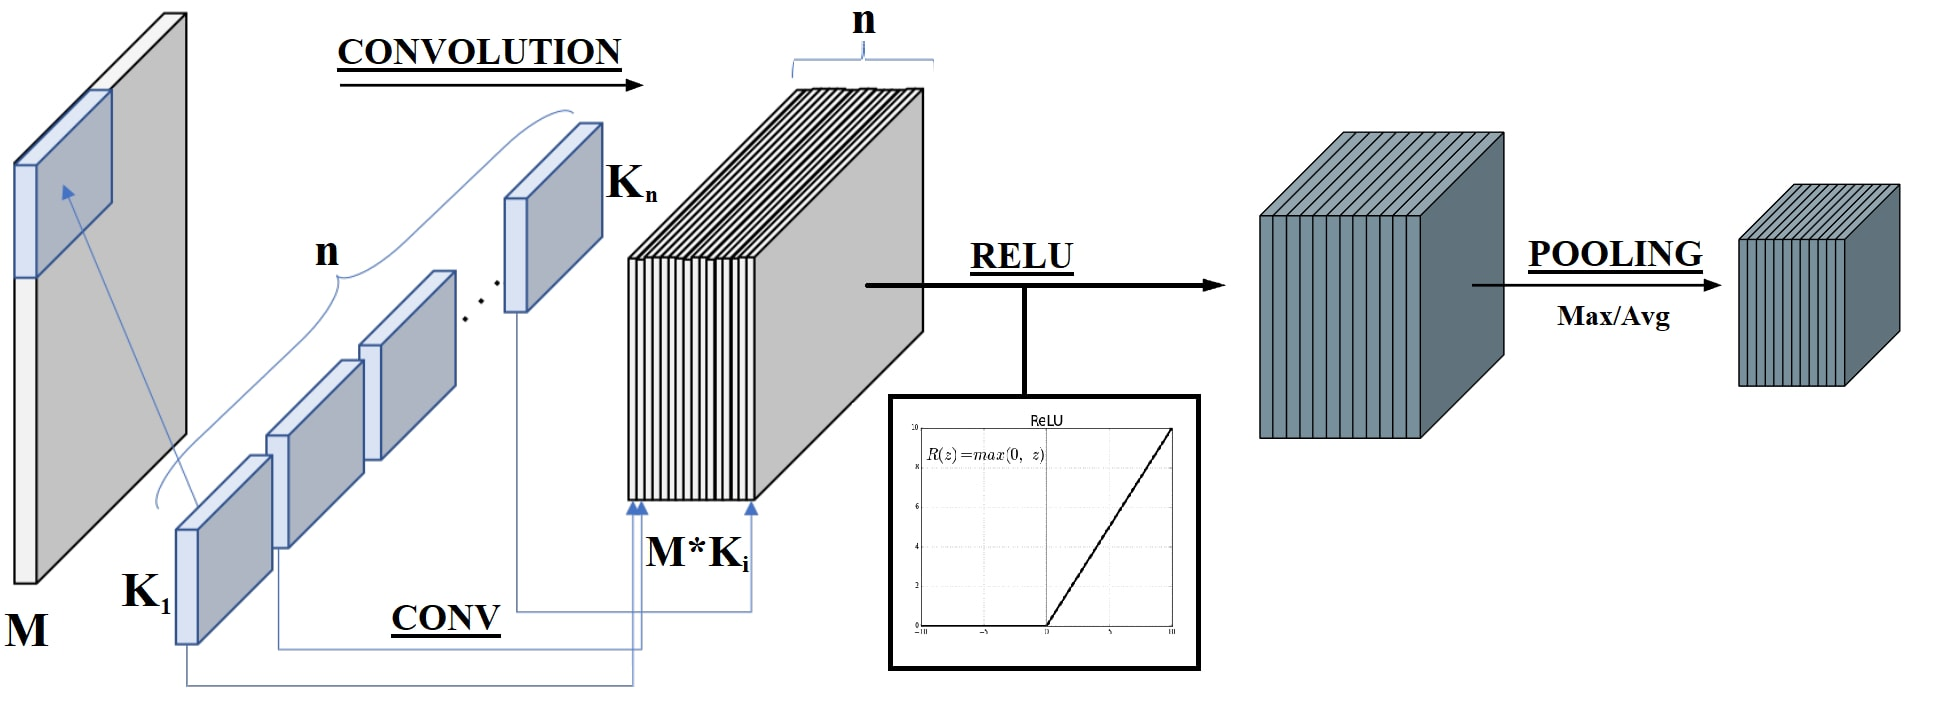
\includegraphics[width=0.85\textwidth]{figures/Conv_RELU_Pool.PNG}\caption{Principe du bloc de convolution}
        \onslide<4>\centering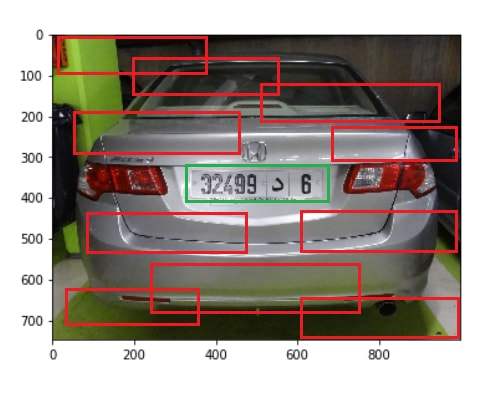
\includegraphics[width=0.37\textwidth]{figures/RCNN.PNG}\caption{Détection par fenêtres glissantes}
    \end{overprint}
\end{figure}
\end{frame}


%%%%%%%%%%%%%%%%%%%%%%%%%%%%%%%%%%%%%%%%%%%%%%%%
% Cinquième diapo
%%%%%%%%%%%%%%%%%%%%%%%%%%%%%%%%%%%%%%%%%%%%%%%%

\begin{frame}
\frametitle{Création du réseau de neurones}
\framesubtitle{Solution Optimale}


\begin{itemize}
    \item<1->   "YOLO" : Une transformation de l'espace du problème
    \begin{itemize}
        \item<2->   Diviser l'image en grilles
        \item<3->   Localiser celle contenant le centre de l'objet.
        \item<4->   Déterminer le vecteur de sortie.
    \end{itemize}
\end{itemize}

\centering
\begin{figure}
    \begin{overprint}
        \onslide<1>\centering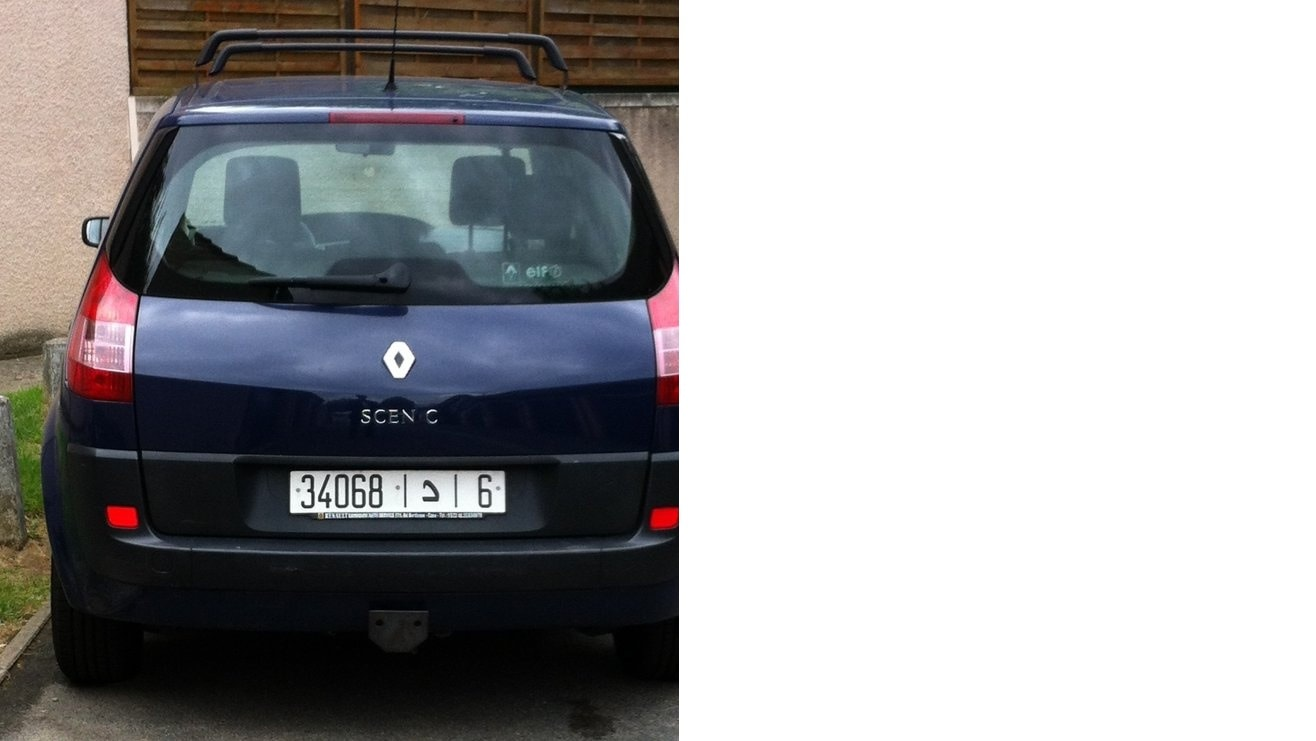
\includegraphics[width=0.6\textwidth]{figures/Car.PNG}\caption{Exemple d'image à traiter}
        \onslide<2>\centering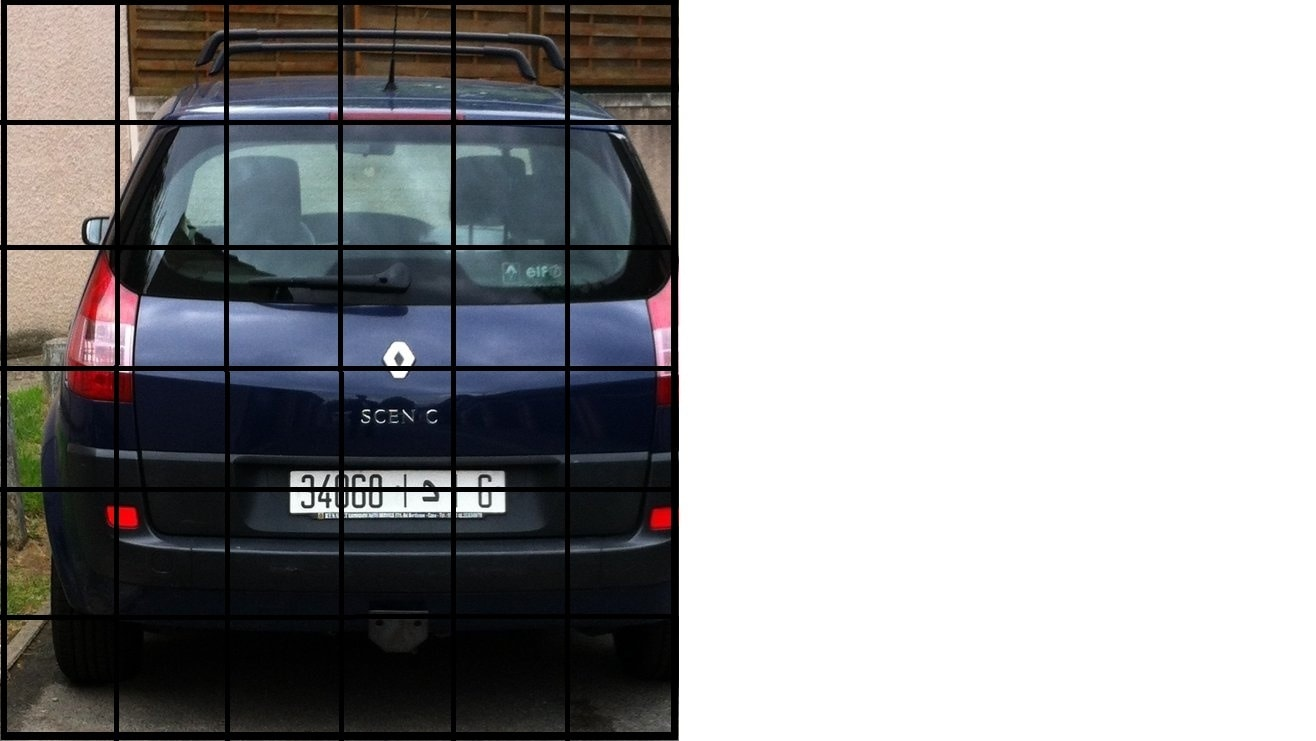
\includegraphics[width=0.6\textwidth]{figures/Grid.PNG}\caption{Première étape}
        \onslide<3>\centering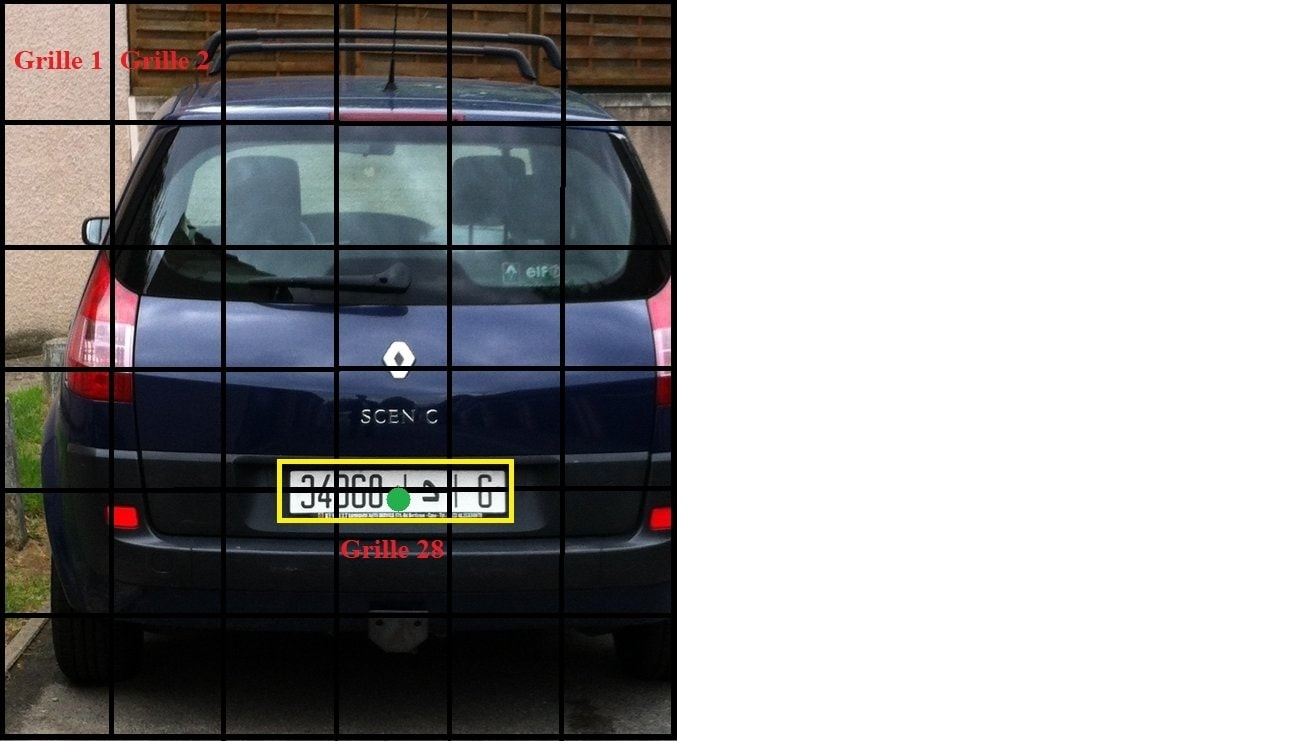
\includegraphics[width=0.6\textwidth]{figures/Center.PNG}\caption{Deuxième étape}
        \onslide<4>\centering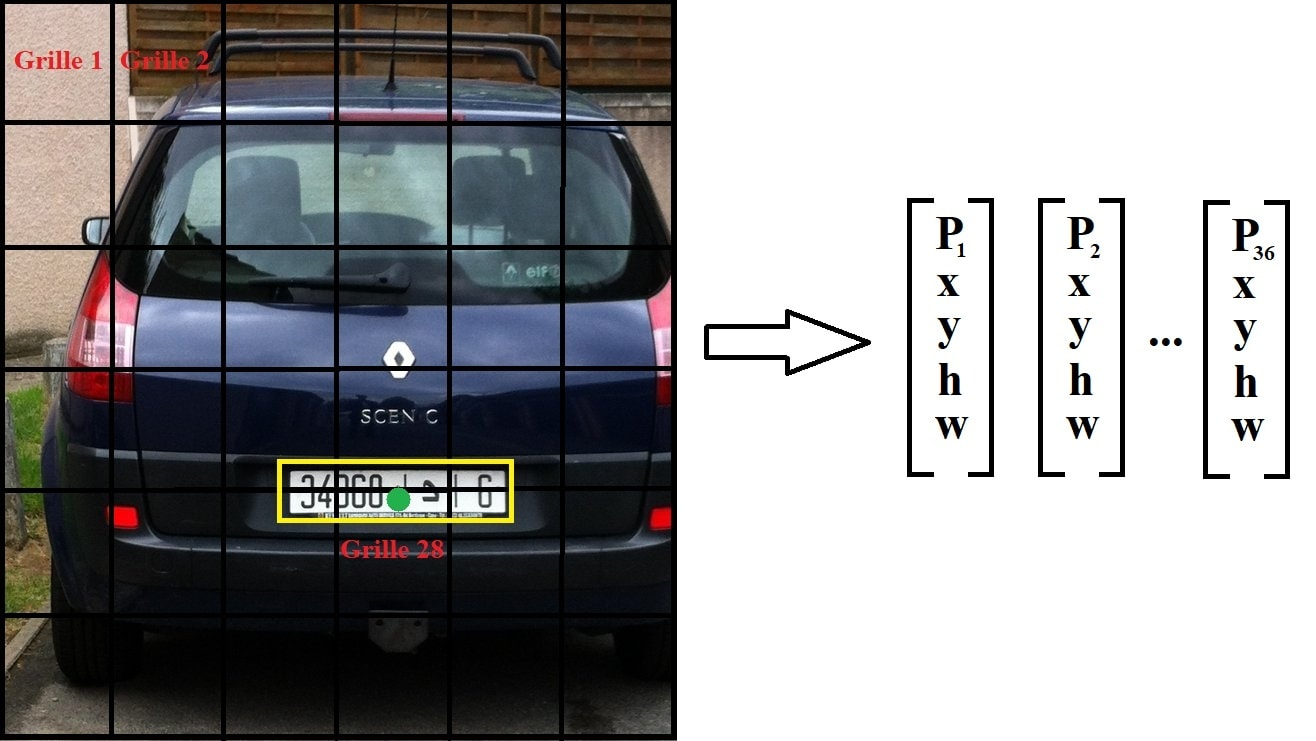
\includegraphics[width=0.6\textwidth]{figures/YOLO.PNG}\caption{Troisième étape}
    \end{overprint}
\end{figure}
\end{frame}

%%%%%%%%%%%%%%%%%%%%%%%%%%%%%%%%%%%%%%%%%%%%%%%%
% Sixième diapo
%%%%%%%%%%%%%%%%%%%%%%%%%%%%%%%%%%%%%%%%%%%%%%%%

\begin{frame}
\frametitle{Création du réseau de neurones}
\framesubtitle{Variété de solutions}

\begin{itemize}
    \item<1->   Differents extracteurs de caractéristiques :
    \begin{itemize}
        \item<1->   DarkNet : Structure originale.
        \item<2->   MobileNet : Développée par Google.
        \item<3->   SqueezeNet : Développée par Stanford.
    \end{itemize}
\end{itemize}
\begin{figure}
    \begin{overprint}
        \onslide<1>\centering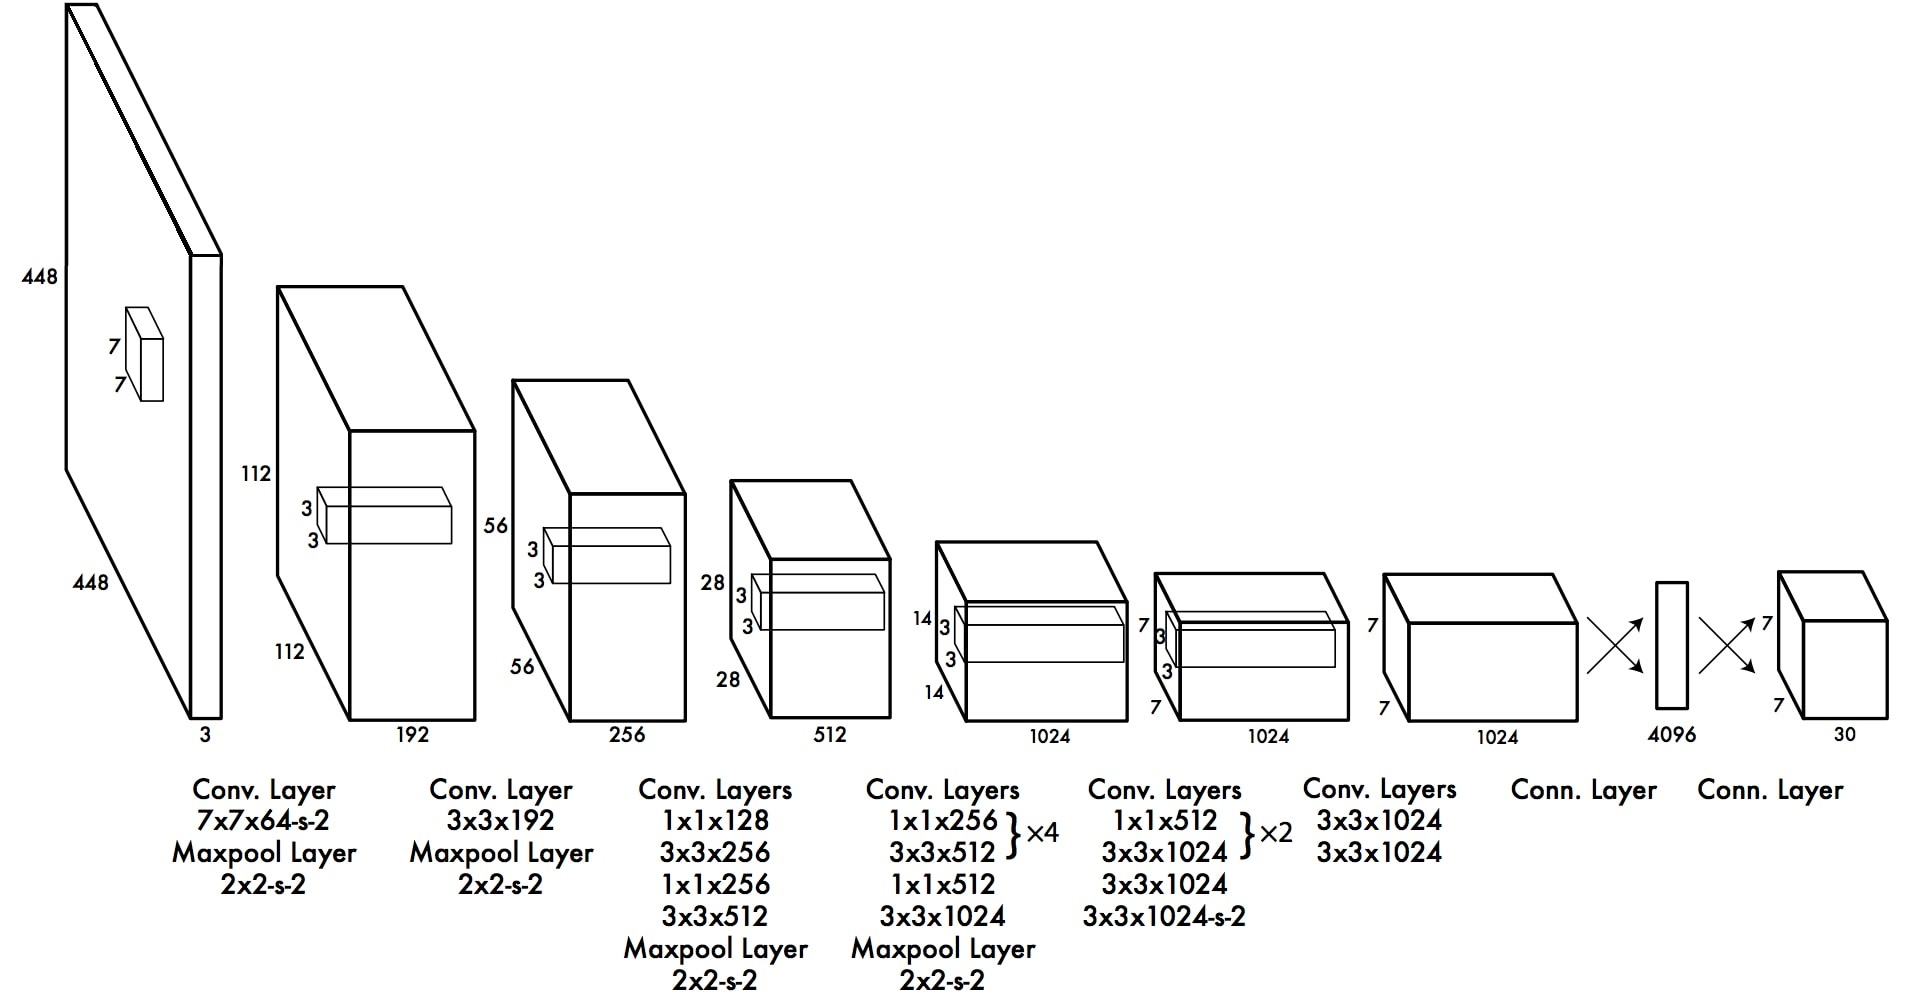
\includegraphics[width=0.67\textwidth]{figures/Darknet.PNG}\caption{Structure globale de DarkNet}
        \onslide<2>\centering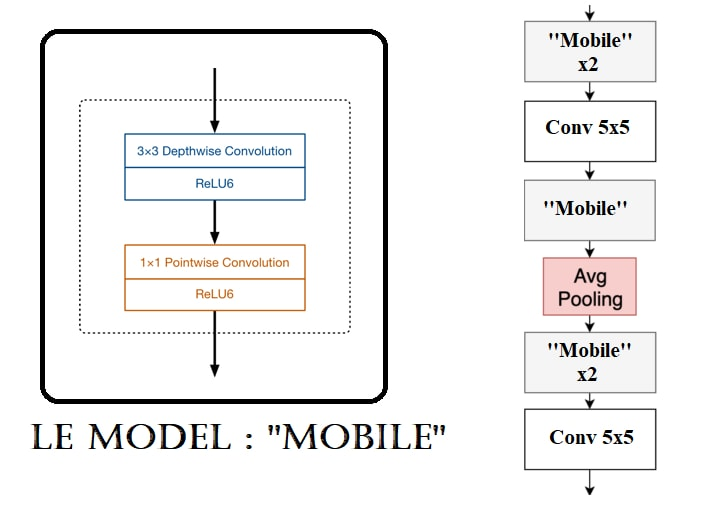
\includegraphics[width=0.45\textwidth]{figures/MobNet.PNG}\caption{Unité principale de MobileNet}
        \onslide<3>\centering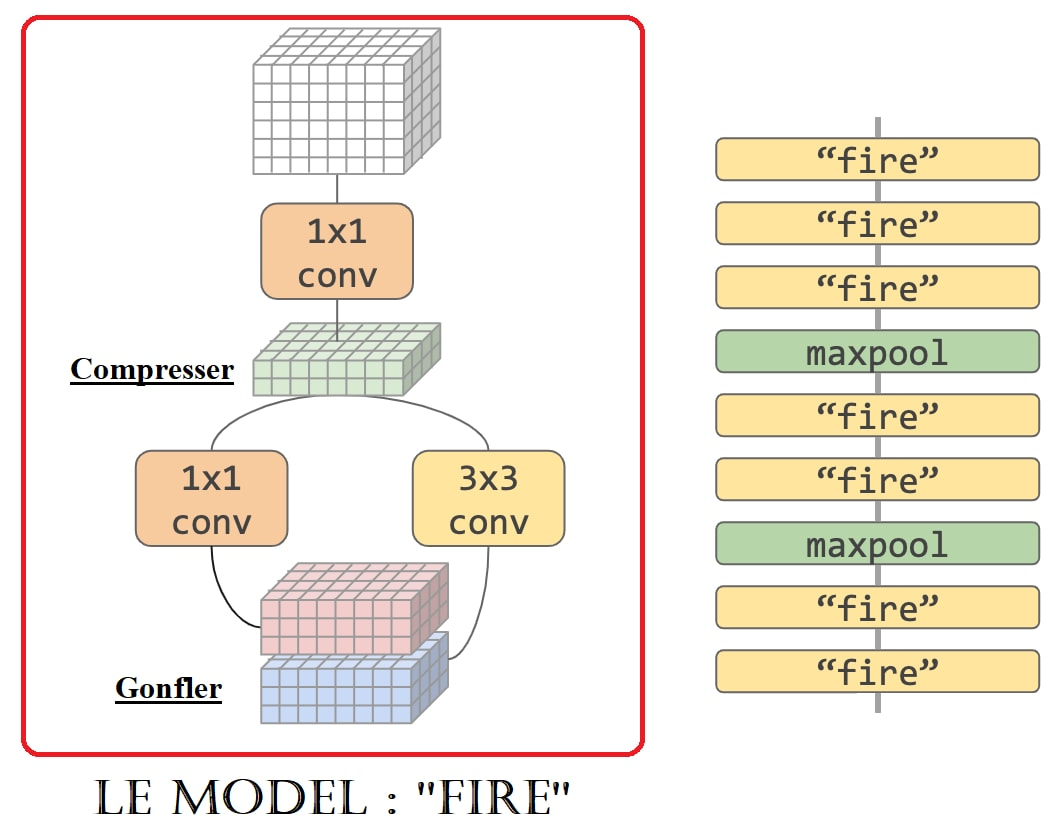
\includegraphics[width=0.42\textwidth]{figures/SqzNet.PNG}\caption{Unité principale de SqueezeNet}
    \end{overprint}
\end{figure}
\end{frame}

%%%%%%%%%%%%%%%%%%%%%%%%%%%%%%%%%%%%%%%%%%%%%%%%
% Septième diapo
%%%%%%%%%%%%%%%%%%%%%%%%%%%%%%%%%%%%%%%%%%%%%%%%

\begin{frame}
\frametitle{Création du réseau de neurones}
\framesubtitle{Comparaison entre structures}

\begin{table}
\begin{tabular}{c|c|c|c}
    Classifieur  &  Nombre de   &  Temps de    &  Temps          \\
                 &  paramètres  &  traitement  &  d'entrainement \\
    \hline
    DarkNet      &  50,983,561  &  0.5  s      &  Plus que 20 jours \\
    MobileNet    &  3,284,214   &  0.09 s      &  6 jours et 3 heures  \\
    SqueezeNet   &  750,198     &  0.02 s      &  1 jours et 14 heures
\end{tabular}
\end{table}
\centering
\begin{figure}
    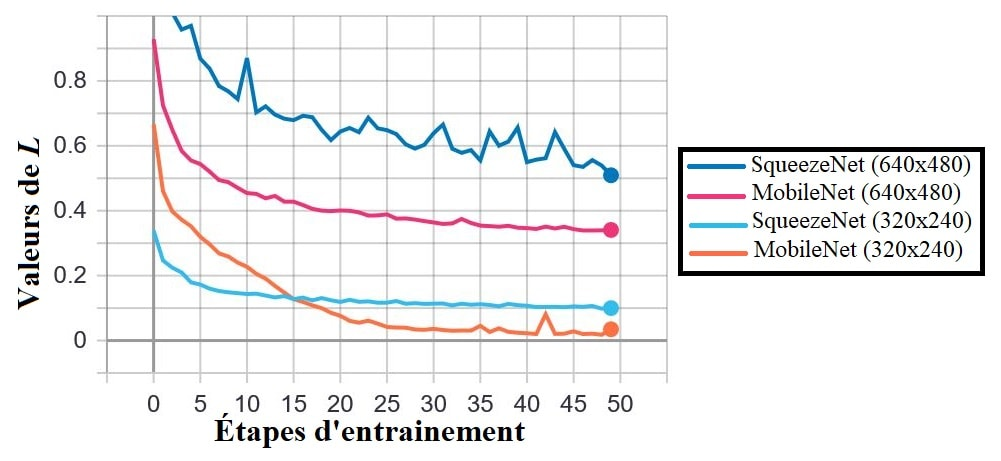
\includegraphics[width=0.55\textwidth]{figures/Epochs.PNG}\caption{Resultats d'entrainement}
\end{figure}
\end{frame}

%%%%%%%%%%%%%%%%%%%%%%%%%%%%%%%%%%%%%%%%%%%%%%%%
% huitième diapo
%%%%%%%%%%%%%%%%%%%%%%%%%%%%%%%%%%%%%%%%%%%%%%%%

\begin{frame}
\frametitle{Création du réseau de neurones}
\framesubtitle{Évaluation de la structure retunue : SqueezeNet}
\captionsetup{justification=centering}
\begin{columns}
\begin{column}{6cm}
    \begin{itemize}
    \item<1->   Sur les images :
    \begin{itemize}
        \item<1->   Bons résultats.
        \item<1->   Bonus : Généralisation.
    \end{itemize}
    \item<2->   Sur un flux vidéo :
        \begin{itemize}
            \item<2->   Détection en temps réel.
            \item<2->   Bonus : Multi-détection.
        \end{itemize}
    \end{itemize}
\end{column}
\begin{column}{6cm}
    \begin{figure}
        \begin{overprint}
        \captionsetup{justification=centering}
            \onslide<1>\centering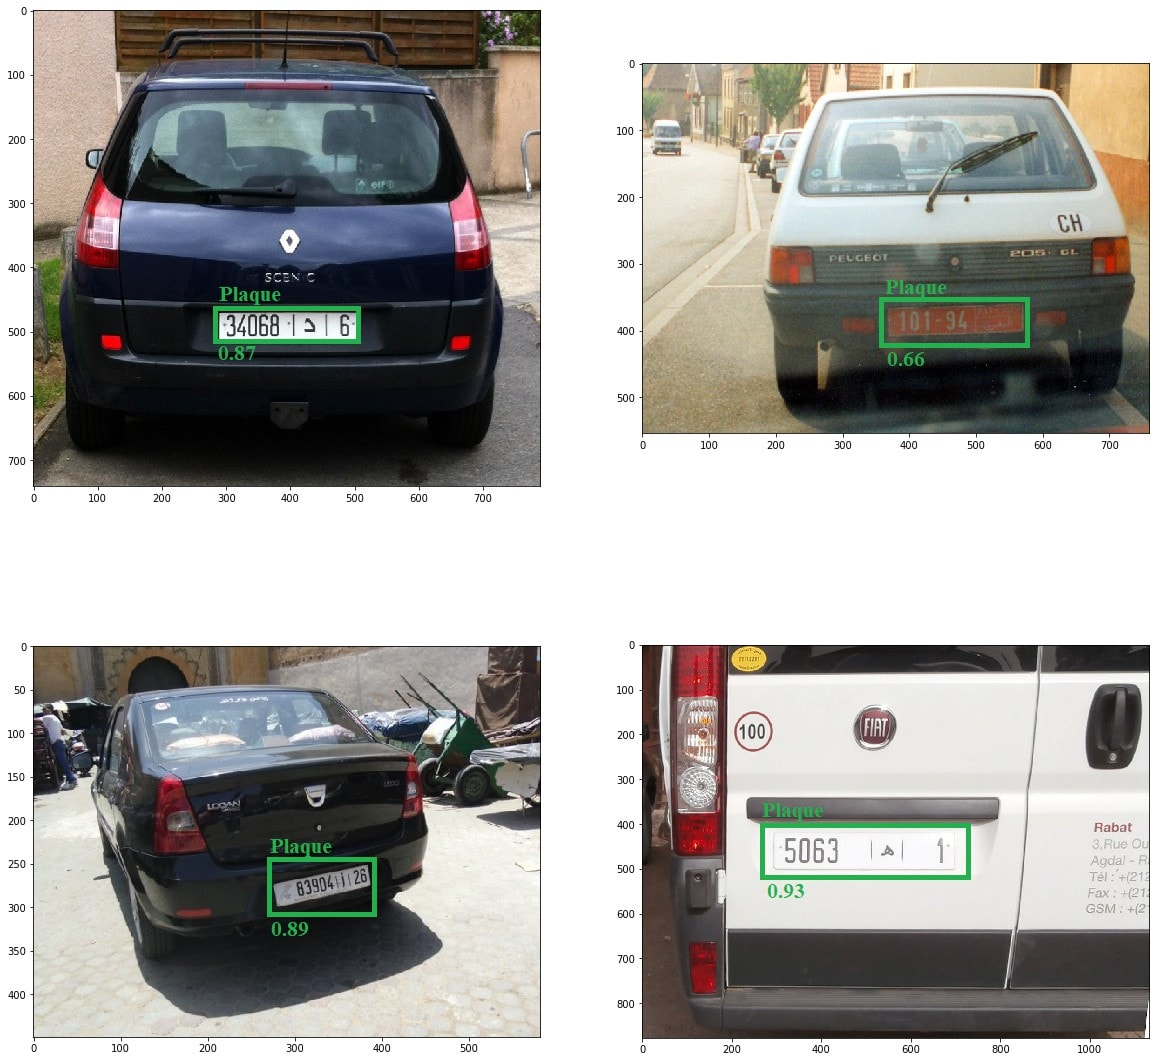
\includegraphics[width=0.8\textwidth]{figures/Eval.PNG}\caption{Exemples de détections dans des cas differents}
            \onslide<2>\centering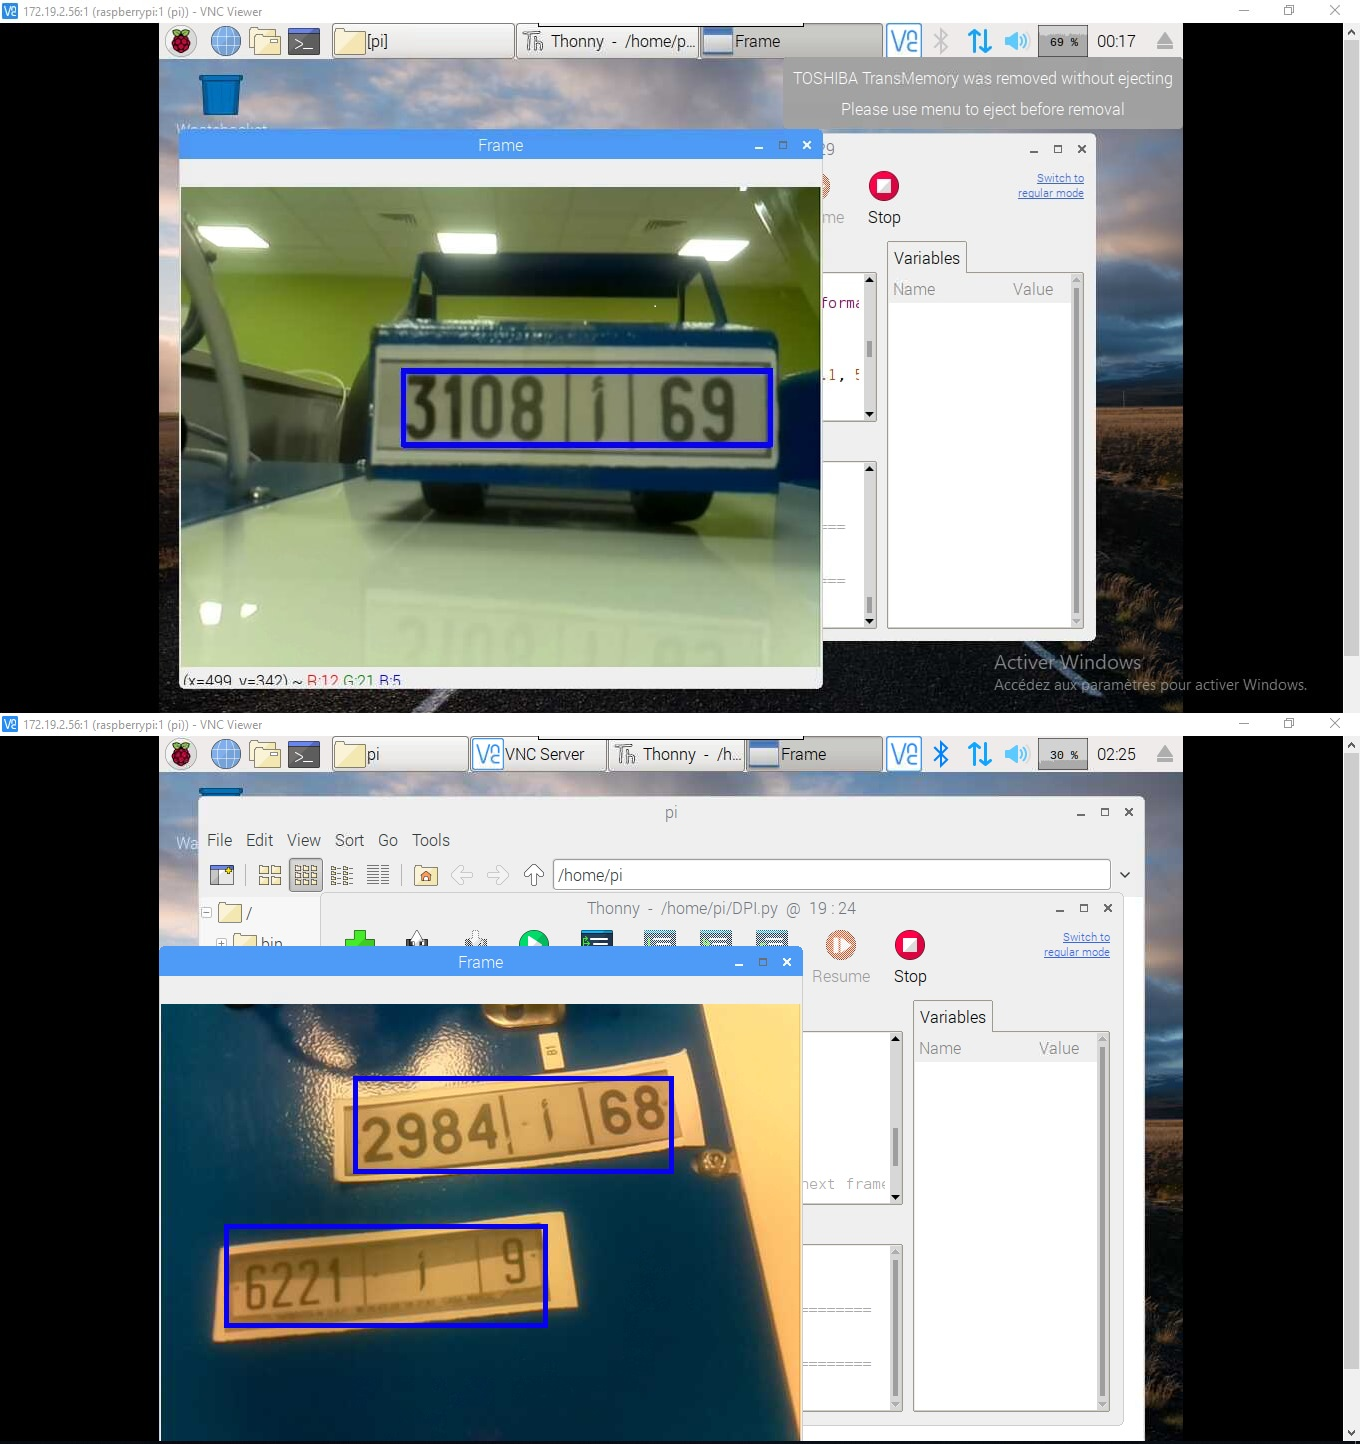
\includegraphics[width=0.8\textwidth]{figures/Stream.PNG}\caption{Resultats avec Raspberry}
        \end{overprint}
    \end{figure}
\end{column}
\end{columns}
\end{frame}